\documentclass{article}
\title{\textbf{Notes on Geometric Learning}}
\author{Matthew Mo}
\date{\today}

\usepackage{ctex, xeCJK, zxjatype}
\usepackage{metalogo, makecell, svg, amssymb, amsfonts, amsmath, physics, fancyhdr, geometry, graphicx, pdfpages, ragged2e, bm}
\usepackage{verbatim}
\newcommand{\R}{\mathbb{R}}
\newcommand{\rarr}{\rightarrow}
\newcommand{\lop}{Laplace算子}
\newcommand{\tRarr}{$\Rightarrow$}
\newcommand{\trarr}{$\Rightarrow$}
\newcommand{\filter}{\Gamma_{l,l'}}
\newcommand{\fn}[1]{\footnote{#1}}
\newcommand{\bs}[1]{\boldsymbol{#1}}
\newcommand{\iprod}[2]{\langle #1, #2 \rangle}
\newcommand{\define}{\textbf{Definition} }
\newcommand{\trm}{\textbf{Theorem} }
\newcommand{\alg}{\textbf{Algorithm} }
\newcommand{\cov}{\text{Cov}}
\newcommand{\bb}{\mathbb}
\newtheorem{theorem}{Theorem}[section]
\newtheorem{lemma}[theorem]{Lemma}
\newtheorem{proposition}[theorem]{Proposition}
\newtheorem{corollary}[theorem]{Corollary}
\newtheorem{definition}[theorem]{Definition}

\newenvironment{proof}[1][Proof]{\begin{trivlist}
\item[\hskip \labelsep {\bfseries #1}]}{\end{trivlist}}
% \newenvironment{definition}[1][Definition]{\begin{trivlist}
% \item[\hskip \labelsep {\bfseries #1}]}{\end{trivlist}}
\newenvironment{example}[1][Example]{\begin{trivlist}
\item[\hskip \labelsep {\bfseries #1}]}{\end{trivlist}}
\newenvironment{idea}[1][Idea]{\begin{trivlist}
\item[\hskip \labelsep {\bfseries #1}]}{\end{trivlist}}
\newenvironment{remark}[1][Remark]{\begin{trivlist}
\item[\hskip \labelsep {\bfseries #1}]}{\end{trivlist}}
\renewcommand{\cal}{\mathcal}
\usepackage[hidelinks, bookmarks]{hyperref} % add index hyper-links
\newcommand{\coro}{\textbf{Corollary} }
\newcommand{\tgt}{\textbf{Target} }
\newcommand{\bt}[1]{\textbf{#1}}
\newcommand{\lp}{Lagrange Polynomial}
\newcommand{\np}{Newton Polynomial}
\newcommand{\where}{\text{where }}
\newcommand{\centerimage}[2]{
    \centerline{\includegraphics[width=#1\paperwidth]{#2}
    }
}
\let\titleoriginal\title           % save original \title macro
\newcommand{\thetitle}{}
\renewcommand{\title}[1]{          % substitute for a new \title
    \titleoriginal{#1}%               % define the real title
    \renewcommand{\thetitle}{#1}        % define \thetitle
}

\newCJKfontfamily\gothic{IPAexGothic}
\newCJKfontfamily\mincho{IPAexMincho}

% set plain style
\pagestyle{fancy}
\lhead{} 
\chead{} 
\rhead{} 
% \lfoot{\it Notes on Geometric Learning} 
\lfoot{\hyperref[contents]{\thetitle}} 
% \lfoot{\thetitle} 
\cfoot{}
\rfoot{\thepage} 


% Length to control the \fancyheadoffset and the calculation of \headline
% simultaneously
\newlength\FHoffset
\setlength\FHoffset{1cm}

\addtolength\headwidth{2\FHoffset}

\fancyheadoffset{\FHoffset}

% these lengths will control the headrule trimming to the left and right 
\newlength\FHleft
\newlength\FHright

% here the trimmings are controlled by the user
\setlength\FHleft{1cm}
\setlength\FHright{0cm}

% The new definition of headrule that will take into acount the trimming(s)
\newbox\FHline
\setbox\FHline=\hbox{\hsize=\paperwidth%
  \hspace*{\FHleft}%
  \rule{\dimexpr\headwidth-\FHleft-\FHright\relax}{\headrulewidth}\hspace*{\FHright}%
}
\renewcommand\headrule{\vskip-.7\baselineskip\copy\FHline}

\renewcommand{\headrulewidth}{0.7pt} % hline width
\renewcommand{\footrulewidth}{0.7pt} 

% set margin
\geometry{a4paper,scale=0.75}
\newcommand{\note}{\textbf{Note} }
\begin{document}
\maketitle
\tableofcontents
\section{Math Backgrounds}
\subsection{Analysis on $\mathbb R ^ n$}

\subsection{Differential Manifold}
一个微分流形(differential manifold)基本上就是一个局部欧式空间的拓扑空间.严格上来说:一个$d$维微分流形$\mathcal{X}$是一个拓扑空间,并且对于每一个其中的点都存在一个邻域与$d$维欧氏空间(i.e. $\mathbb{R}^d$)同胚(homoemorphic),称作切空间(tangent space)$T_x\mathcal{X}$,所有切空间一起(的并)组成了切丛(tangent bundle)$T\mathcal{X}$,并且可以定义内积$\langle \cdot, \cdot \rangle_{T_x\mathcal{X}}:T_x\mathcal{X}\times T_x\mathcal{X} \rightarrow \mathbb{R}$,关于$x$是光滑的,成为流形上的一个黎曼度量(Riemann metric).后文中的流形若非特殊指出意味着微分流形.一个流形和其上的黎曼度规称为黎曼流形.注意,以上定义中的任何定义都是内蕴的,图也可以是一个流形!

\textbf{Target} 将在欧氏空间上大获成功的CNN方法推广到流形(以及图)上!

\textbf{Theorem}(Whitney weak embbeding theorem) 任意$n$维微分流形$M$可以光滑地嵌入$\mathbb{R}^{2n+1}$,以及光滑的浸入$\mathbb{R}^{2n}$.并且每个连续映射$M\rightarrow \mathbb{R}^{2n+1}$($M\rightarrow \mathbb{R}^{2n+1}$)可以用光滑嵌入(浸入)逼近,也即这些光滑嵌入(在所有连续映射中)是稠密的.

一个更强的定理指出,任意$n$维微分流形$M$可以光滑地嵌入$\mathbb{R}^{2n}$,但它们不再稠密.

\textbf{Theorem}(Nash embedding theorem) 任意Riemann流形可以保距地光滑嵌入某个维度的欧氏空间中.

\subsection{Calculus on Manifold}
我们关心两种流形上的函数:标量场$f:M\rightarrow \mathbb{R}$,切向量场$F:M\rightarrow TM$.可以定义流形上函数的内积,这让平方可积函数形成Hilbert空间:
\begin{align}\langle f, g\rangle_{L^2(M)}=\int_M f(x)g(x) dx\end{align}
\begin{align}\langle F, G\rangle_{L^2(TM)}=\int_M \langle F(x)G(x) \rangle_{L^2(M)} dx
\end{align}
其中$dx$是Riemann度量诱导的体积微元.

$f$的微分是一个算子:$df:TM\rightarrow \mathbb{R}$
作用在切向量场上,在$x\in M$上,微分可以被定义为一个1-形式:
\begin{align}
    df(x)=\langle \nabla f(x), \cdot \rangle_{T_x M}
\end{align}
以及导数
\begin{align}
    df(x)F(x)=\langle \nabla f(x), F(x) \rangle_{T_x M}
\end{align}
这是一种方向导数的推广.有内蕴导数(梯度)
\begin{align}
    \nabla f:L^2(M)\rightarrow L^2(TM)
\end{align}
对称地有它的形式伴随算子内蕴散度
\begin{align}
    div f :L^2(TM)\rightarrow L^2(M)
\end{align}
因为$$\langle F(x), \nabla f(x) \rangle_{L^2(TX)}=\langle -div F(x), f(x) \rangle_{L^2(X)}$$

Laplace-Beltrami算子:$\Delta f=-div \nabla f$.它是自伴(对称)算子.

Dirichlet能量:$||\nabla f||_{L^2(TM)}=\langle \nabla f, \nabla f \rangle_{L^2(TM)}=\langle f, \Delta f \rangle_{L^2(M)}$衡量了一个函数的光滑程度

注意:以上定义无关流形地外含性质,是内蕴地定义.于是我们可以通过在切空间上定义一个基,并且用$d$-向量表示切向量,以及$d\times d$对称矩阵表示Riemann度规.

\subsection{Graph and Discrete Differential Operators}
考虑带权无向图$(\mathcal{V},\mathcal{E})$,以及边和点权
\begin{align}
    \begin{cases}
        w_{ij} \ge 0,\forall (i,j)\in \mathcal E\\
        a_i > 0 ,\forall i\in \mathcal V
    \end{cases}
\end{align}
定义其上的内积并给出Hilbert空间:
\begin{align}
    \begin{cases}
        \langle f, g \rangle_{L^2(\mathcal V)}=\sum_{v\in \mathcal V}a_if_ig_i\\
        \langle F, G \rangle_{L^2(\mathcal E)}=\sum_{e\in \mathcal E}w_{ij}F_{ij}G_{ij}
    \end{cases}
\end{align}
图梯度$\nabla:L^2(\mathcal V)\rightarrow L^2(\mathcal{E})$:
\begin{align}
    \nabla f_{ij}=f_i-f_j
\end{align}
图梯度$\nabla:L^2(\mathcal E)\rightarrow L^2(\mathcal{V})$:
\begin{align}
    div F_{i}=\frac{1}{a_i}\sum_{(i,j)\in \mathcal{E}}w_{ij}F_{ij}
\end{align}
图Laplace算子$\Delta:L^2(\mathcal V)\rightarrow L^2(\mathcal{V})$:
\begin{align}
    \Delta f=-div \nabla f
    \Delta f_i=\frac{1}{a_i}\sum_{(i,j)\in \mathcal{E}}w_{ij}(f_i-f_j)
\end{align}
下设$\mathbf{W}=(w_{ij}),\mathbf{A}=Diag(a_i),\mathbf{f}=(f_i)^T,\mathbf{D}=Diag(\sum_{j,j\neq i}w_{ij})$
则
\begin{align}
    \Delta f=\mathbf{A}^{-1}(\mathbf{D}-\mathbf{W})\mathbf{f}
\end{align}
$\mathbf{A}=\mathbf{I}\rightarrow$unnormalized graph Laplacian.\\
$\mathbf{A}=\mathbf{D}\rightarrow$randomwalk graph Laplacian.

\subsection{Fourier Analysis on Manifolds}
$\Delta$是自伴,半正定算子,在紧域上有正交特征值分解,记它们是$\phi_0,\dots$,并且其中有$\langle \phi_i, \phi_j \rangle_{L^2(M)}=\delta_{ij}$和对应非负特征值$0\le \lambda_0\le \lambda_1 \le \dots$($\Delta$的谱).
 
\textbf{Idea} $\phi_i$是黎曼流形上最光滑的函数(在Dirichlet能量意义上),可以作为Fourier分析(Hilbert空间)的基!

计算$f\in L^2(M)$的展开:
\begin{align}
    f(x)=\sum_{i\ge 0}\langle f,\phi_i(x)\rangle_{L^2(M)}\phi_i(x)
\end{align}
在欧式域上的卷积有性质:
\begin{align}
    \widehat{(f*g)}(\omega)=\hat{f}(\omega)\hat{g}(\omega)
\end{align}
但是在非欧域上不能简单地定义卷积($\tau-x$怎么定义?),那么可以由卷积性质定义卷积:
\begin{align}
    \left( f\ast g\right) \left( x\right) =\sum _{i\geq 0} \langle f,\phi _{i} \rangle_{L^2(M)} \langle g,\phi _{i} \rangle_{L^2(M)} \phi _{i}\left( x\right) 
\end{align}
但缺乏平移不变性! 

在图上,Laplace算子有n个特征值向量,并且
\begin{align}
    f*g \Rightarrow \mathbf{G}f=\Phi diag(\mathbf{\hat{g}}) \Phi^T f
\end{align}
其中$\widehat {g}=\left( \widehat {g}_i \right)$是谱表示,$\Phi=(\phi_i)$是Laplace算子的特征矩阵.

\textbf{Note} 卷积和Laplace算子交换$\Delta \mathbf{G} f=\mathbf{G} \Delta f$.

\textbf{Note} \lop 的特征向量组可能不是唯一的(比如符号取反即可),同构域也可能有不同的基,这代表着域结构的小扰动会导致特征向量组的巨大变化,这会导致基于它们的算法难以跨域.有些kernel似乎没有这些问题(heat kernel, diffusion kernel).



\section{Vanilla GNN(Scarselli et al.)}

\bt{Target} node $v$ \trarr  representation $\bs h_v \in \R^s$ \trarr  out $\bs o_v$

\bt{Domain} undirected graph + node feature $\bs x_v$ + possible edge feature.

$co[v], ne[v]$:edges, neighbors of $v$.

\subsection{Model} 
\begin{align}
    \label{upd1}
    h_v&=f(x_v, x_{co[v]}, h_{ne[v]}, x_{ne[v]})\\
    o_v&=g(h_v,x_v)
\end{align}
where $f$:local transition function, $g$: local out function, both parametric. Let $\bs{H, O, X, X_N}$ are those states in mat form
\begin{align}
    \bs H&=F(\bs H, \bs X)\\
    \bs O&=F(\bs H, \bs X_N)
\end{align}
$F$:global transition function, $G$: global out function, both parametric, use fixed point iteration to calculate $\bs H$:
\begin{align}
    \bs H^{t+1}&=F(\bs H^t, \bs X)
\end{align}
write loss using supervisory target info $t_i$
\begin{align}
    loss=\sum_{i=1}^p(t_i-o_i)
\end{align}
$p$ is node count supervised.

\note An Implicit Neuron Representation!

\alg 
\begin{enumerate}
    \item update $h'_v$ from (\ref{upd1}) for $T$ time steps
    \item compute loss and gradients
    \item update parameters
\end{enumerate}

\note equals $T$ layers of GNN of same parameters
 
\subsection{Limitations}

\begin{itemize}
    \item computational inefficient
    \item each layer share same parameters\tRarr goto either RNN(GRU/LSTM)/ use different params
    \item edge features?
    \item large $T$ \trarr graph representation be smooth, hard to distinguish nodes
    \item \bt{Further Nets} 
    \begin{itemize}
        \item GGNN(computational efficiency)
        \item R-GCN(directed graph)
    \end{itemize}
\end{itemize}

\section{Spectral Methods}

\subsection{Spectral CNN(SCNN, Bruna et al.)}
一个谱卷积层:
\begin{align}
    g_l=\xi\left(\sum_{l'=1}^p \Phi_k \filter \Phi_k^T f_{l'}\right)
\end{align}
其中:
\begin{itemize}
    \item $\xi$是某种非线性函数,如$ReLU, tanh, sigmoid$
    \item $F=(\mathbf f_1, \mathbf{f_q})\in K^{n\times q},G=(\mathbf g_1,...,\mathbf g_p)\in K^{n\times p}$是p/q个I/O信号(在图的顶点上,$n=|\mathcal{V}|$)
    \item $\filter\in K^{k\times k}$是一个对角阵,代表了频域的一个滤波器
    \item $\Phi_k$是前$k$个特征向量组成的矩阵,代表了只用了前k个特征向量的截止频率,一般应用中$k\ll n$
    \item $\bs \Delta=\bs I - \bs D^{-\frac{1}{2}} \bs A \bs D^{-\frac{1}{2}}$, 利用的是normalized \lop.
\end{itemize}
这种方法:
\begin{itemize}
    \item 仅限于单一域:$\filter$取决于基的选取.
    \item 可以在跨域上建立正交基,但需要域的先验知识,如域之间的对应,然而后者常常是难以找到的
    \item 设$k=O(n)$个特征向量被保留,则一个卷积层中有$pqk=O(n)$个参数,如果让$k=O(1/n)$则可以使之类似于CNN,参数数和输入大小无关!
\end{itemize}

\subsection{Graph Coarsening}
图粗化就是池化的类比:以$\alpha<1$的比例保持图顶点,那么令$\Phi,\widetilde{\Phi}$是$n\times n, \alpha n \times \alpha n$的特征值矩阵,则有
\begin{align}
    \widetilde{\Phi}\approx P\Phi\left(\begin{array}{ccc}
        I_{\alpha n}\\
        0
    \end{array}\right)
\end{align}
其中$P\in\{0,1\}^{\alpha n\times n}$,其中i行编码了第i顶点在粗化图中的位置.然而由于应用了非线性,要在粗化后每层计算特征矩阵.

\textbf{Note} 单个高频分量$\Rightarrow$不稳定,把高频分量组合$\Rightarrow$有意义的信息.

\subsection{Spectral CNN + 光滑谱滤波器}
为了降低overfit,需要降低参数个数:亟需限制谱乘子的类别($\filter$),在频域上表达局域性.

在欧式空间上有Pascal恒等式:
\begin{align}
    \int_{\R}|x|^{2k}|f(x)|^2dx=\int_{\R}\left|\frac{\partial^k \widetilde{f}(\omega)}{\partial\omega^k}\right|d\omega
\end{align}

\textbf{Idea} \begin{itemize}
    \item 学一个时域局域化filter\tRarr 学一个光滑filter
    \item 在一个频率的子集上学习谱乘子,再内插(如三次样条)!
\end{itemize} 

有
\begin{align}
    diag(\filter)=\mathbf{B}\boldsymbol{\alpha}_{l,l'}
    \gamma_i=\sum_{j=1}^q \alpha_j \beta_j(\lambda_i)
\end{align}
其中$\mathbf{B}=(b_{ij})=(\beta_j(\lambda_i))\in \R^{k\times q}$是固定的内插kernel(如$\beta_j(\lambda)$是三次样条),$\boldsymbol{\alpha}$是$q$个内插系数.

若选择$n\gamma^{-1}=O(1)$个内插系数,使参数与$n$无关,总模型有$O(\log n)$个可训练参数(why?).但是BP/FP的复杂度仍然很高,这是由于$\boldsymbol{\Phi_k}$和$\boldsymbol{\Phi_k}^T$的乘法复杂度很高,在欧式域上有FFT算法,是$O(n\log n)$的,但是在普通意义上的图上没有此类算法,只能$O(n^2)$.\tRarr 接下来会看到避免此计算的方法.

\section{Non-Spectral Methods}

\textbf{Idea} \lop 的多项式在特征值上相同地作用,故可以用多项式展开代替在特征值上的作用:
\begin{align}
    &g_\alpha(\Delta)=\boldsymbol{\Phi}g_\alpha (\boldsymbol{\Lambda})\boldsymbol{\Phi}^T,\\
    &g_\alpha(\lambda)=\sum_{j=0}^{r-1}\alpha_j \lambda^j\\
    &\boldsymbol{\Lambda}=diag(\lambda_i)
\end{align}
此时$\filter=g_{\alpha_{l,l'}}(\bs{\Lambda})$,自动生成局域化filter.由于$\Delta^r$是$r$-局域化的,所以上面的filter就像是作用在r-hops上的diffusion kernel.
\subsection{Graph CNN(GCNN a.k.a. ChebNet, Defferard et al.)}

使用Chebyshev多项式:
\begin{align}
    T_0(\lambda)&=1,
    T_1(\lambda)=\lambda,\\
    T_j(\lambda)&=2\lambda T_{j-1}(\lambda)-T_{j-2}(\lambda)\\
    T_n(x)&=\cos(n \acos(x))
\end{align}

展开filter:
\begin{align}
    g_\alpha(\tilde \Delta)
    &=\sum_{j=0}^{r-1}\alpha_j \bs{\Phi}T_j(\tilde{\bs{\Lambda}})\bs{\Phi}^T
    =\sum_{j=0}^{r-1}\alpha_j T_j(\tilde{\Delta})
\end{align}
其中$\tilde{\Delta}=2\lambda_n^{-1} \Delta-\bs{I},\tilde{\bs{\Lambda}}=2\lambda_n^{-1} \bs{\Lambda}-\bs{I}$,代表了$[0,\lambda_n]\Rightarrow[-1,1]$的归一化.

记$\bar f^{(j)}=T_j(\tilde{\Delta})f$,可计算
\begin{align}
    \bar f^{(j)}&=2\tilde \Delta \bar f^{(j-1)}-f^{(j-2)}\\
    \bar f^{(1)}&=\tilde \Delta \bar f\\
    \bar f^{(0)}&=f
\end{align}
这是$O(rn)$的,并且无需显式计算\lop .
以及总filter:
\begin{align}
    g_\alpha(\tilde \Delta) f
    &=\sum_{j=0}^{r-1}\alpha_j T_j(\tilde{\bs \Delta}) f\\
    &=\sum_{j=0}^{r-1}\alpha_j \bar f^{(j)}
\end{align}
每层:
\begin{align}
    y_{s,i}=\sum_{j} g_{\alpha_{i,j}}(\widetilde{\bs \Delta})x_{s_j}
\end{align}

采用的图粗化技术(Graclus):在每一级图粗化水平上,我们遍历结点,当i结点遍历到时,找一个邻接点使得局部割$W_{ij}(1/d_i+1/d_j)$最小化;两个匹配结点被合并为一个,标记已遍历并权值相加.实行这种池化操作时,会得到一个平衡二叉树,这里,若一个结点只有一个子节点,那么给它增加一个fake node,并初始化其上的信号为0,且不与其它节点相连.


\subsection{Graph Convolutional Net(GCN, Kipf, Welling et al.)}

\textbf{Idea} 简化GCNN的设定:$r=2,\lambda_n\approx 2$,
这给出
\begin{align}
    g_\alpha(f)
=\alpha_0 f+\alpha_1(\Delta - \bs{I})f
=\alpha_0 f+\alpha_1\mathbf{D}^{-1/2}\mathbf{W}\mathbf{D}^{-1/2}f
\end{align}

\textbf{Idea} 更进一步$\alpha=\alpha_0=-\alpha_1$,
这给出
\begin{align}
    g_\alpha(f)=\alpha (\bs{I}+\mathbf{D}^{-1/2}\mathbf{W}\mathbf{D}^{-1/2})f
\end{align}
又由于$(\bs{I}+\mathbf{D}^{-1/2}\mathbf{W}\mathbf{D}^{-1/2})$的元素取值于$[0,2]$,会导致数值不稳定,所以重整化之:
\begin{align}
    g_\alpha(f)=\alpha \widetilde{\mathbf{D}}^{-1/2}\widetilde{\mathbf{W}}\widetilde{\mathbf{D}}^{-1/2}f
\end{align}
其中$\widetilde{\mathbf{W}}=\bs{W}+\bs{I},\widetilde{\mathbf{D}}=diag(\sum_{j\neq i}\tilde w_{ij})$, TC.: $O(|\mathcal{E}|FC)$

为了解决半监督图学习问题,可以通过带正则\lop 项的损失函数来训练:
\begin{align}
    L=L_0+\lambda L_{reg}, L_{reg}=\sum_{i,j}A_{ij} ||f(X_i)-f(X_j)||^2=f(X)^T\bs{\Delta}f(X)
\end{align}
其中第一项是有监督的损失项\tRarr 带了一个先验假设:相邻顶点相似.用GCN直接在有监督损失上训练可以避免这个先验.

\subsection{Adaptive GCN/AGCN, [Li et al., 2018b]}

\tgt 学习隐含的结点关系.

\bt{Idea} 学习一个residual \lop: $\widehat{\bs L} = \bs L + \alpha \bs L_{res}$,$\bs L_{res}$学习得到:
\begin{align}
    &\bs L_{res} = \bs I - \widehat{\bs D}^{-\frac{1}{2}} \widehat{\bs A} \widehat{\bs D}^{\frac{1}{2}}\\
    &\widehat{\bs D} = deg(\widehat{\bs A})
\end{align}
其中$\widehat{\bs A}$学得:
\begin{align}
    &G_{x_i,x_j}=\exp(-D(x_i,x_j)/2\sigma^2)\\
    &D(x_i, x_j)=\sqrt{(x_i-x_j)^T M(x_i-x_j)} \text{(Mahalanobis dist.)}
\end{align}
其中$\bs M$是学得的参数,满足$\bs M=\bs W_d^T \bs W_d$

\subsection{Graph Neural Net(GNN)}

\textbf{Note} ChebNet, GCN可以看作是在图的r/1-hops上作用,是GNN的特例!

\textbf{Idea} 一个GNN在不同层上学一个高/低通算子:$f\rightarrow Wf$,$f\rightarrow \Delta f$.

对于每个顶点上一个$p$-维向量的图信号$\bs F$,GNN考虑一个非线性函数$\eta_\theta:\R^p\times\R^p\rightarrow\R^q$应用在每个图顶点上,$g_i=\eta_\theta((\bs W f)_i,(\bs D f)_i)$,
令$\eta(a,b)=b-a$给出\lop,$\eta$的选择给出不同任务适用的diffusion kernel.

\begin{itemize}
    \item 连续应用同一个卷积层$c_\theta=g_\theta(f)$ \tRarr 动力系统的稳态
    \item Coarsening \tRarr 单一输出
    \item 可用于实现其它图上的算子
\end{itemize}

\section{Charting-based Methods}

\textbf{Problem} 在不同域上进行同种操作?
但是定义的卷积难以在不同域上推广\tRarr 定义另一种卷积!

考虑欧式卷积,它涉及一个一个pixel移动kernel并作乘法,图上对应?结构没有平移不变性!流形/图上缺少全局参数化\tRarr 寻找内蕴坐标 \tRarr 图册和局部坐标系!

\textbf{Idea} 寻找权函数$v_{1\dots J}(x,\cdot)$,那么定义
\begin{align}
    \label{d1}
    D_j(x)f=\int_Mf(x')v_j(x,x')dx'
\end{align}
这提供了内蕴的卷积
\begin{align}
    \label{d2}
    (f*g)(x)=\sum_j g_jD_j(x)f
\end{align}
这里$g$是应用在patch上的各系数,参数个数$O(J)=O(1)$.

\subsection{Geodesic CNN(测地CNN)}

\textbf{Idea} 使用切空间上自带的极坐标
$$\rho_(x')=d(x,x'),\theta(x')=\dots$$
那么权函数
\begin{align}
    v_{ij}(x,x')=e^{-(\rho(x')-\rho_i)^2/2\sigma_\rho^2}e^{-(\theta(x')-\theta_j)^2/2\sigma_\theta^2}
\end{align}
其中$i=1,\dots,J,j=1,\dots,J'$是半径/角度的个数,把patch拆分为了$J J'$个bin,且大小为$\sigma_\rho\times \sigma_\theta$


\subsection{Anisotrophic CNN(各向异性CNN)}

\textbf{Idea} 使用各向异性的扩散核:
\begin{align}
    f_t(x,t)=-div(A(x)\nabla f(x,t))
\end{align}
其中$A$是热导率张量,在2d情形时为$2\times2$矩阵

一个选择:\begin{align}
    \bs A_{\alpha\theta}=R_\theta \left(\begin{array}{ccc}
        \alpha  &\\
           &1
    \end{array}\right)R_\theta^T(x)
\end{align}
其中$R_\theta$是按照某个轴(如最大曲率轴)的旋转.对应的heat kernel:
\begin{align}
    h_{\alpha\theta t}(x,x')=\sum_{i\geq 0}\exp(-t\lambda_{\alpha \theta i})\phi_{\alpha \theta i}(x)\phi_{\alpha \theta i}(x')
\end{align}
其中$\phi_{\alpha \theta 0}(x),..$是特征函数,$\lambda_{\alpha \theta i}$是对应特征值,of各向异性\lop$\Delta_{\alpha \theta}f(x)=-div(A_{\alpha \theta}(x)\nabla f(x))$

\subsection{Dynamic Graph CNN(DGCNN)}

\bt{Idea} 使用MLP学习一个权重函数\trarr EdgeConv block | 用k-NN建立点云的图表示.

对于两个点$x_i, x_j\in \R^F$,计算边权$h_\Theta(x_i,x_j)$(e.g. use MLP),并在点上对相连的边做聚合操作$\Box$(some mean/sum/max etc.)得到$F'$维的顶点特征:
\begin{align}
    x'_i=\Box_{(i,j)\in \mathcal{E}} h_\Theta(x_i,x_j)
\end{align}
一个经典选择是patch上的卷积:
\begin{align}
    x_{im}'=\sum_m \theta_m \cdot x_j
\end{align}
m是channel序号,
另几种:
\begin{align}
    h(x_i,x_j)=\begin{cases}
        &h(x_i), \text{or}\\
        &h(x_j), \text{and Guassian kernel(权重)}\\
        &h(x_j-x_i)\\
        &\bar h(x_i, x_j-x_i)
    \end{cases}
\end{align}
这种方法(DGCNN)里:
\begin{align}
    &e'_{ijm}=ReLU(\theta_m \cdot (x_j-x_i)+\phi_m x_i)\\
    &x'_{im}=\max_j e'_{ijm}
\end{align}

\note 每次进行了一次卷积之后,重新构建(这里是k-NN)图结构\trarr 动态性.并且,这卷积操作具有形变不变性和平移不变性(如果$\phi \equiv 0$),具体网络架构采用了Dense-Conn.思想(之前的层全部连接到fc层上):
\begin{figure}[t]
    \centering
    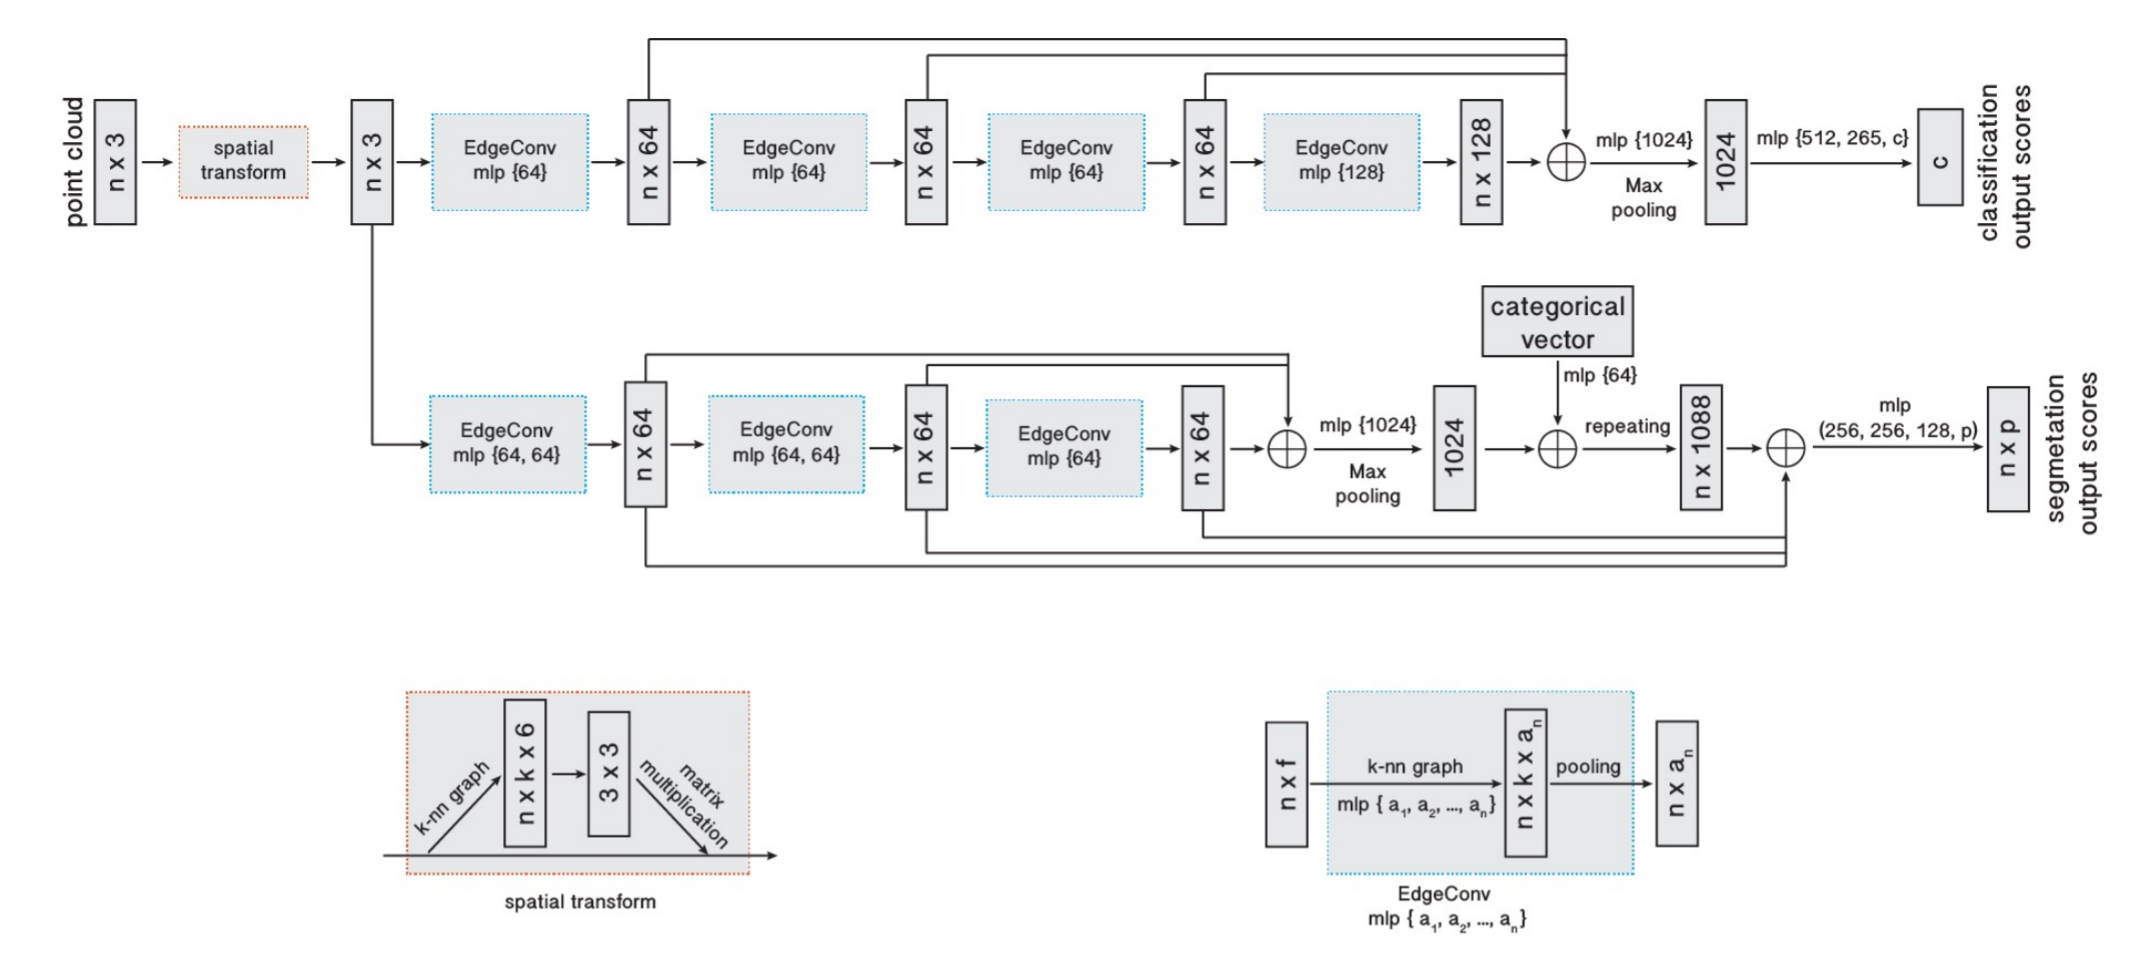
\includegraphics[width=0.85\paperwidth]{dgcnn_structure.PNG}
    \caption{Structure of DGCNN}
\end{figure}



\subsection{Mixture Model Network(MoNet, Monti et al.)}

\textbf{Idea} 在图册上定义局部坐标系$\bs u_x(x')$,在这些坐标上应用一些带参数的kernel$[v_{1\dots J}(\bs u)]$以形成权函数.

采用Gaussian核:
\begin{align}
    v_j(\bs u)=\exp(-\frac{1}{2} (\bs u - \bs \mu_j)^T \bs \Sigma_j^{-1} (\bs u - \bs \mu_j))
\end{align}
参数是$J$个$\bs \Sigma \in \R^{d\times d}$和$\bs \mu\in \R^{d\times 1}$.

实践中,这些更大的自由度\tRarr 很多问题的SOTA方法

\section{Spatial Methods}

\subsection{Neural FPS (Duvenaud et al., 2015)}

\bt{Idea} different node degrees \trarr different weights
\begin{align}
    &x=h_v^{t-1}+\sum_{i=1}^{|N_v|}h_i^{t-1}\\
    &h^t_v=\xi(x\bs W_t^{|N_v|})\\
    &\text{where }\bs W_t^{|N_v|} \text{ is weights on layer $t$ of node deg. $|N_v|$}
\end{align}

\bt{Limitation} Can't go large-scale

\subsection{PATCHY-SAN (Niepert et al., 2016)}

\bt{Idea} 选择并正则化正好k个邻接点(可以不是1-hop上的,若不够),这些点送到卷积层去进行计算

\begin{enumerate}
    \item \bt{Node Seq. Selection} 用某种图标号过程将图排序,谭厚选择一个处理图节点的顺序,然后按照stride $s$选取结点,直到选取了$w$个结点.(不一定包含所有结点)
    \item \bt{Neighborhood Assembly} 对于上述序列中的每个结点,使用BFS得到k个邻接点.
    \item \bt{Graph Norm.} 试图给感受野中的结点一个顺序.参见原论文!
    \item \bt{Conv. Architecture} 接着就可以送到CNN中,其中正则化了的邻域就是感受野,边/顶点特征维度就是channels.
\end{enumerate}

\subsection{Diffusion-Convolutional NN/DCNN(Atwood and Towsley, 2016)}

\bt{Idea} 对于结点分类,有
\begin{align}
    \bs H=\xi(\bs W^c \odot \bs P^* \bs X)
\end{align}
其中$\bs X:N\times F, \bs P^*=\{\bs P^{i}\}_i:N\times K \times N,\bs P$是度正则化的转移矩阵(deg.-norm. transition mat.) , $\bs H$是图顶点的diffusion-representation.

\subsection{Dual GCN/DGCN(Zhuang and Ma, 2018)}

\bt{Idea} 分别考虑全局和局部一致性,使用两个CNN,第一个即GCN,第二个将邻接矩阵替换成了PPMI(positive pointwise mutual info.)矩阵(两个网络共享权重!):
\begin{align}
    \bs H'=\xi(\bs D_P^{-1/2} \bs X_P \bs D_P^{1/2}\bs H \bs \Theta)
\end{align}
其中$\bs X_P$是PPMI矩阵,$\bs D_P$是对应度矩阵.

\bt{Motivations of 2nd Net} 类似context的结点应该有类似表示.

我们把这两个CNN分别称为$Conv_A$和$Conv_P$,那么可以把两个网络集成在一个loss下
\begin{align}
    L=L_0(Conv_A)+\lambda(t) L_{reg}(Conv_A,Conv_P)
\end{align}其中$\lambda(t)$是动态平衡因子,$L_0(Conv_A)$是有监督的loss(通过结点label),若网络的输出是$Z^A$,softmax化后是$\widehat Z^A$,那么可以写出
\begin{align}
    L_0(Conv_A)=-\frac{1}{|y_L|}\sum_{l\in y_L}\sum_{i=1\dots C} Y_{i,l}\ln\left(\widehat Z^A_{i,l}\right)
\end{align}
另一边的loss
\begin{align}
    L_{reg}(Conv_A,Conv_P)=\frac{1}{n}\sum_{i=1\dots n}||\widehat Z^A_{i,:}-\widehat Z^P_{i,:}||^2
\end{align}

\subsection{Learnable GCN/LGCN(Gao et al.,2018)}

\bt{Idea} 基于LGCL(Learnable Graph Conv. Layer)和子图学习策略.LGCL提升CNN作集成器,在邻接矩阵上作max-pooling,得到top-k特征元素并送到1-d CNN上得到repr.,具体FP过程:
\begin{align}
    &\widehat{H_t}=g(H_t,A,k)\\
    &{H_{t+1}}=c(\widehat{H_t})
\end{align}
其中$A$是邻接矩阵,$g$是选择最大$k$个结点的op,$c$是卷积层.

关于g: 给定结点x,设它有n个邻接点,特征是c维的,
% !TODO

\section{Spatial-Spectral Methods}

\subsection{Windowed Fourier Transform}

\textbf{Idea} 传统傅里叶变换由不确定性原理限制,时域局部性\tRarr 难以达成频域局域性\tRarr 带窗傅里叶变换(Windowed Fourier Transform, WFT, Short-Time FT, Spectrogram)

WFT:(on $\R^n$,$g(x)$是窗口函数)
\begin{align}
    (Sf)(x,\omega)&=\int_\R f(x')g(x'-x)e^{-i\omega x'}dx'\\
    &= \iprod{f}{g_{x,\omega}}_{L^2(\R)}\\
    \text{where }&g(x'-x)e^{-i\omega x'}=g_{x,\omega}(x')
\end{align}
拓展到非欧域上,要定义平移算子为和$\delta$函数的卷积:
\begin{align}
    (g*\delta_{x'})(x)&=\sum_{i\ge 0} \iprod{g}{\phi_i}_{L^2(M)} \iprod{\delta_{x'}}{\phi_i}_{L^2(M)} \phi_i(x)\\
    &=\sum_{i\ge 0} \widehat{g_i} \phi_i(x')\phi_i(x)
\end{align}
那么就可以写出非欧域上的WFT atoms:
\begin{align}
    g_{x',j}(x)=\phi_j(x')\sum_{i\ge 0} \widehat{g_i} \phi_i(x')\phi_i(x)
\end{align}
这里window大小被Fourier系数$\widehat{g_i}$确定.给出WFT:
\begin{align}
    (Sf)(x',j)=\iprod{f}{g_{x',j}}_{L^2(M)}=\sum_{i\ge 0} \widehat{g_i} \phi_i(x')\iprod{f}{\phi_i\phi_j}_{L^2(M)}
\end{align}

\textbf{Note} 这些定义都是内蕴的!

\subsection{Wavelet Transform}

\textbf{Idea} 频域分解\tRarr 尺度分解 \tRarr 小波分解

\textbf{Target} 定义时/频域上局域性都很好的小波基,可用于还原/近似信号

一个简单实现:Haar小波.\\
Learning: 找到个尺度上的最优的结点配对\tRarr 多项式复杂度!

\subsection{Localized Spectral CNN (LSCNN, Boscaini et al.)}

\textbf{Idea} 用(\ref{d1}),(\ref{d2})之中的卷积,但是利用WFT定义patch:
\begin{align}
    D_j(x)f = (Sf)(x,j)
\end{align}

\section{Application}

\begin{itemize}
    \item 网络分析
    \begin{itemize}
        \item 文献引用图(CORA)
        \item ranking \& community detection | 求解特征值/Fiedler向量,包含了最小割的信息. 
        \item PageRank: 通过借一个改动的 \lop 的特征值来rank.
    \end{itemize}
    \item 推荐系统
    \begin{itemize}
        \item 矩阵补全问题 \tRarr Geometric CNN
        \item (Monti et al.) Multi-Graph CNN + RNN: 由MGCNN提取的特征送到RNN作为对score的更新.
    \end{itemize}
    \item CV/CG
    \begin{itemize}
        \item 3d-geometric data processing: rasterizing可行,但是会丢失拓扑信息
        \item CG(Mesh Correspondence/Classification)
    \end{itemize}
    \item 粒子物理和化学
    \item 分子设计
    \item 医学影像
\end{itemize}

\section{Open Problems and Discussions}


\begin{itemize}
    \item Generalization
    \begin{itemize}
        \item 谱方法: 难以跨域
        \item 时域方法/图册方法: 定义适当的局部坐标系较难
    \end{itemize}
    \item 时变域: 动态形状, abnnormal social events
    \item 有向图: \lop 不是对称的,没有正交特征值分解
    \item 生成问题: 如何从内蕴的结构/表示重建几何结构
    \item 计算效率问题: 非欧域上的DL常常没有网格结构,难以在GPU上高效计算
\end{itemize}



\end{document}